\documentclass[a4paper,12pt,twoside,english,openany]{book}
[a4paper,12pt,twoside]
\usepackage[icon=Note,color=yellow,author=Sepand]{pdfcomment}
\usepackage[utf8]{inputenc}
\usepackage[T1]{fontenc}
\usepackage{babel}
\usepackage[a4paper,left=3cm,right=2.5cm,top=3cm,bottom=3cm, twoside]{geometry}
\usepackage{xcolor}
\usepackage{stmaryrd}
\usepackage{amssymb}
\usepackage{amsmath}
\usepackage{libertine}
\usepackage[
    natbib=true,
    style=numeric,
    sorting=none
]{biblatex}

\addbibresource{res/biblio.bib} 

\usepackage{caption}
\usepackage{subcaption}
\usepackage{float}
\usepackage{multirow}
\usepackage{array, multirow, tabularx}
\usepackage{booktabs}
\usepackage{longtable}
\usepackage{apalike}
\usepackage{minitoc}
\usepackage{tikz}
\usetikzlibrary{calc, positioning, arrows.meta,arrows, shapes.geometric}
\usepackage[strict]{changepage}
\usepackage{siunitx}
\usepackage{enumitem}
\usepackage{epigraph}
\usepackage{lscape}
\usepackage{titletoc}
\usepackage{mdframed}
\usepackage{tabu}
\usepackage{pdfpages}
\usepackage{arydshln}
\usepackage{calc}
\usepackage{titlesec} 
\usepackage{sectsty}
\usepackage{lipsum}
\usepackage{emptypage}

\usepackage{fancyhdr}
\pagestyle{fancy}
\usepackage{graphicx}
\graphicspath{ {res/} }
\usepackage{hyperref} 
\hypersetup{
    colorlinks=true,
    linkcolor=black,
    filecolor=black,      
    urlcolor=black,
    citecolor=black,
    }
\definecolor{linkColor}{HTML}{32a852}

\titleformat{\chapter}[hang]
  {\normalfont\bfseries}{}{0pt}{\Huge}


%\sectionfont{\color{CentraleRed}}  % sets colour of sections
%\subsectionfont{\color{uclablue}}  % sets colour of subsections, ou gray, teal 
\definecolor{darkseagreen}{rgb}{0.56, 0.74, 0.56}

\title{Multimodal MRI-PET Imaging: Estimation of Image-Derived Arterial Input Function in Brain PET Imaging \\ Application to Modeling PET Dynamics of Glucose Metabolism in Patients with Impaired Consciousness}
\author{Sepand Ali Madad Soltani}
\date{January 2025}



\leftmark 
\rightmark 


\usepackage[xindy]{imakeidx}
% \makeindex
%\input{auxilliaires/glossaire}

\begin{document}

\begin{titlepage}
	\begin{center}
		\begin{tabular}{c@{\hskip 7cm}c@{\hskip 1cm}}
			\includegraphics[height=3cm]{res/ucbl.png} &
			\includegraphics[height=3cm]{res/polytech.png}
		\end{tabular}
	\end{center}

	\begin{center}

		\vspace*{.03\textheight}
		\textsc{\Large University of Claude Bernard Lyon 1 }\\[0.2cm]
		\large Polytech Lyon

		\rule{\textwidth}{0.8pt} \\
		\vspace{10pt}

		{\Large \bfseries Multimodal MRI-PET Imaging:
			Estimation of Image-Derived Arterial Input Function in Brain PET Imaging
			Application to Modeling PET Dynamics of Glucose Metabolism in Patients with Impaired Consciousness
		}
		\rule{\textwidth}{0.8pt} \\

	\end{center}

	\vfill
	\begin{center}
		By \textsc{\Large Sepand Ali Madad Soltani}\\[1cm]
		Master's Thesis Report\\[1.2cm]
		Supervised by \textsc{\large Inés Mérida}
		and
		\textsc{\large Nicolas Costes}  \\[0.2cm]
		Academic Advisor: \textsc{\large Kevin Tse Ve Koon}\\[0.2cm]
		November 2024 - January 2025

	\end{center}

	\vspace{1cm}
\end{titlepage}

\renewcommand{\chaptermark}[1]{\markboth{#1}{}}


\frontmatter
\chapter*{Abstract}
\paragraph*{Keywords:}PET, Image-Derived, ...

\tableofcontents

\mainmatter
\setlength{\parskip}{.7em}

\renewcommand{\baselinestretch}{1.1}


\fancyhead[]{}
\fancyfoot[]{}
\fancyhead[LH]{\leftmark}
\fancyhead[RH]{\thepage}

\chapter{Introduction}

\section{Positron Emission Tomography Imaging}
explain dynamic pet
\cite{Faulkes2013}

\lipsum[1-1]
\section{Dynamic PET and TAC Modeling}
\lipsum[1-1]
\section{Need for Input Function in PET}
\lipsum[1-1]

\section{Image Derived Input Function}
\lipsum[1-1]


\chapter{Materials and Methods}

\section{Dataset Description}
We utilized a dataset of 56 comatose patients, aged between  X and Y years, in which dynamic PET imaging was conducted 90 minutes using 18FDG as the tracer, with arterial blood sampling and TOF-MRA images acquired during the same session.
\pdfcomment{Do i need to say the age or mention more details?}
\section{Carotid Segmentation\label{sec:carotid}}
Since vessels appear as hypersignal in TOF-MRA, a high-intensity thresholding technique was employed.
First, a threshold value was computed by selecting all nonzero intensity values outside the brain mask and determining a high quantile of these intensities.
Only voxels exceeding this threshold and located outside the brain mask were retained.
Next, a region-growing step was applied to refine the initial selection, ensuring that continuous vascular structures were captured as the final carotid mask.

In addition to arteries, venous structures and lesions may also appear as hypersignal and might be selected by the algorithm.
To exclude them, a cuboid mask was defined in a reference image covering the neck area, where the carotids are most likely to appear.
This mask was first registered to the MRA image and then applied to the uncorrected carotid mask to exclude unwanted tissues.


\begin{figure}
	\centering
	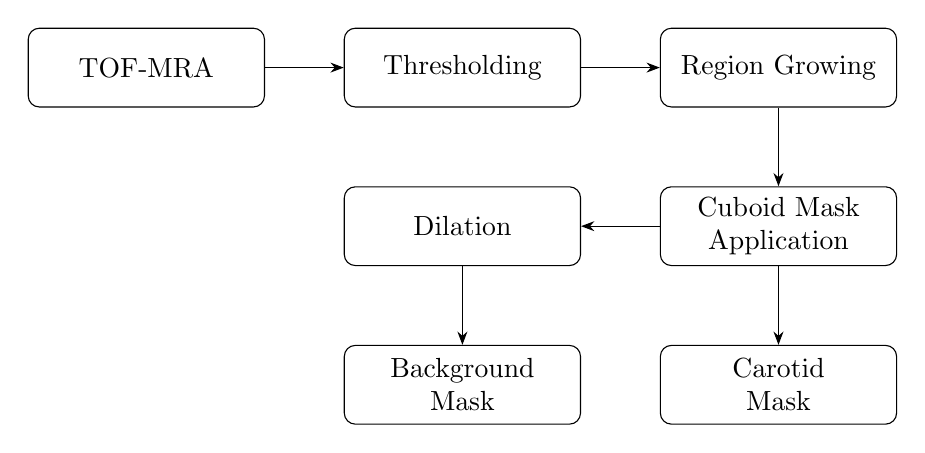
\begin{tikzpicture}[
			node distance=1cm,
			auto,
			>=Stealth,
			mybox/.style={draw, rounded corners, rectangle, minimum width=3cm, minimum height=1cm, align=center}
		]
		\node[mybox] (input) {TOF-MRA};
		\node[mybox, right=of input] (thresh) {Thresholding};

		\node[mybox, right=of thresh] (grow) {Region Growing};
		\node[mybox, below=of grow] (exclude) {Cuboid Mask\\Application};
		\node[mybox, left=of exclude] (dilation) {Dilation};
		\node[mybox, below=of exclude] (mask) {Carotid\\Mask};
		\node[mybox, below=of dilation] (bg_mask) {Background\\Mask};

		\draw[->] (input) -- (thresh);
		\draw[->] (thresh) -- (grow);
		\draw[->] (grow) -- (exclude);
		\draw[->] (exclude) -- (mask);
		\draw[->] (exclude) -- (dilation);
		\draw[->] (dilation) -- (bg_mask);
	\end{tikzpicture}
	\caption{Carotid and background mask segmentation pipeline}
\end{figure}

\section{Partial Volume Correction}
\subsection{Geometric Transfer Matrix}
Direct quantification with the IDIF extracted from the MRI mask of the carotids is impractical due to the strong Partial Volume Effects (PVE) in PET images. % explain PVE 
This however can be corrected by the use of the Geometric Transfer Matrix (GTM) method. This method considers the observered TAC to be the linear combination of the true real value and the other effecting regions.
Here we define two regions, the carotids and the background mask which was generated by dilating the carotid mask by 5 pixels and subtracting the voxels corresponding to the carotid mask.

\begin{equation}
	\underbrace{
		\begin{bmatrix}
			T_{c} \\
			T_{bg}
		\end{bmatrix}
	}_{\text{Observered}}
	=
	\underbrace{
		\begin{bmatrix}
			\omega_{c \rightarrow c}  & \omega_{bg \rightarrow c}  \\
			\omega_{c \rightarrow bg} & \omega_{bg \rightarrow bg}
		\end{bmatrix}
	}_{\text{Geometric Transfer Matrix}}
	.
	\underbrace{
		\begin{bmatrix}
			T_{IF} \\
			T_{tissue}
		\end{bmatrix}
	}_{\text{Unknown}},
\end{equation}

where $\omega_{n \rightarrow m}$ is the spill coefficient of region $n$ onto region $m$, which is obtained by convolving the binary mask of region $n$ with the system's point spread function and integrating the resulting intensity over region $m$, normalized by the total signal in region $m$.
where
\begin{equation}
	\omega_{n\to m} = \frac{\displaystyle \int_{\Omega_m} \bigl( h \ast \chi_n \bigr)(\mathbf{r})\,d\mathbf{r}}{\displaystyle \int_{\Omega_m} \bigl( h \ast \chi_m \bigr)(\mathbf{r})\,d\mathbf{r}},
\end{equation}
with \(\chi_n\) and \(\chi_m\) denoting the binary masks of regions \(n\) and \(m\), respectively, \(h\) the system's point spread function, and \(\Omega_m\) the spatial domain of region \(m\).

$T_{c}$ and $T_{bg}$ are respectively the observered carotid and background TACs and $T_{IF}$ and $T_{tissue}$ are the real unknown TACs of the carotid (the input function) and the background tissue.

By inversing the GTM, this system of equations can be easily solved. However, the GTM being a low rank matrix makes the inversion sensitive to noise and biased on small regions such as carotids.
\pdfcomment{more justification on why we need bgtm instead??}

\subsection{Bayesian Geometric Transfer Matrix}
To overcome challenges posed to GTM method, we utilized a Bayesian framework that jointly estimates the input function and tissue kinetics.
For each subject, $C_{IF}$ is modeled as a linear combination of a population mean and its principal components.
These components are derived by performing principal component analysis (PCA) on a set of AIFs collected from the population. Specifically, for each subject, a subset of 10 random subjects is selected from the dataset—excluding the subject under study—to construct the PCA model.
\begin{equation}
	C_{IF}(t) = \mu(t) + \theta_{1} v_{1}(t) + \theta_{2} v_{2}(t) + \theta_{3} v_{3}(t),
\end{equation}
where \(\mu(t)\) is the population mean AIF, \(v_{i}(t)\) are the principal components obtained from PCA, and \(\theta_{i}\) are the subject-specific weighting coefficients.

The background TAC is then generated by convolving this modeled input function with an impulse response function defined by a two-tissue compartment model \cite{jouvie2013estimation}.

\begin{equation}
	C_{bg}(t) = C_{IF}(t) \circledast f(t; K_1, k_2, k_3),
\end{equation}

where $K_1$, $k_2$, and $k_3$ are kinetic parameters of the two-tissue compartment model denoted by $f$.

Parameter estimation is performed using a Metropolis-within-Gibbs Markov Chain Monte Carlo (MCMC) sampler, which explores the posterior distribution of both the kinetic parameters and the PCA coefficients.
In the Bayesian framework \cite{irace2021bayesian}, all model parameters are collected into the vector $\Theta$. The posterior distribution of $\Theta$ given the observed data $\mathcal{D}$ is expressed as
\begin{equation}
	p(\Theta \mid \mathcal{D}) \propto p(\mathcal{D} \mid \Theta) \pi(\Theta),
\end{equation}

where \( p(\mathcal{D} \mid \Theta) \) is the likelihood function and \( \pi(\Theta) \) is the prior distribution over the parameters \( \Theta = (\theta_{1}, \theta_{2}, \theta_{3}, K_{1}, k_{2}, k_{3}) \). The maximum a posteriori (MAP) estimate of \( \Theta \) is given by:

\begin{equation}
	\hat{\Theta}
	=
	\arg\max_{\Theta}
	\left\{
	\ln p(\mathcal{D} \mid \Theta)
	+
	\ln \pi(\Theta)
	\right\}.
\end{equation}
% This Bayesian formulation naturally incorporates prior knowledge and accounts for uncertainties in both the input function and tissue kinetics, resulting in robust parameter estimates.
% In this approach $C_{IF}$ is modeled as a linear combination of the mean and principal components. They were obtained via a population based principal components analysis (PCA) of AIFs. For each subject, $N=10$ subjects were chosen randomally from the dataset (exclude the subject itself) 
% propose a Bayesian framework  In this approach, the true carotid TAC (i.e., the input function) is modeled as a linear combination of a population-derived mean and principal components obtained via PCA on manually sampled AIFs.
%
% Parameter estimation is performed using a Metropolis-within-Gibbs Markov Chain Monte Carlo (MCMC) sampler, which explores the posterior distribution of both the kinetic parameters and the PCA coefficients.
% By integrating the GTM into the likelihood formulation, the method directly accounts for partial volume effects while also leveraging prior information from the population. The resulting maximum a posteriori (MAP) estimates yield a robust, corrected image-derived input function (IDIF) that mitigates the biases and noise sensitivities inherent in the direct inversion of the GTM.

\section{FDG Quantification}
To accurately evaluate the performance of the estimated IDIF against the gold standard AIF, we performed absolute quantification using a two-tissue compartment model (2TCM) \cite{TODO}.

\subsection{Two-Tissue Compartment Model}
2TCM consists of three total compartments and two tissues:
\begin{itemize}
	\item \textbf{Plasma compartment} \((C_p)\): The concentration of tracer in the plasma or blood.
	\item \textbf{Tissue compartment 1} \((C_1)\): The concentration of free (non-metabolized) tracer in tissue.
	\item \textbf{Tissue compartment 2} \((C_2)\): The concentration of receptor-bound tracer in tissue.
\end{itemize}
Rates of transfer between these compartments are defined by the rate constants \(K_1, k_2, k_3\), and \(k_4\).

\begin{figure}[H]
	\centering
	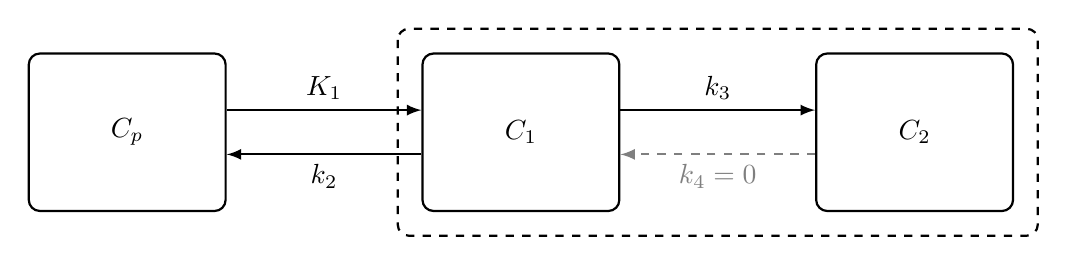
\begin{tikzpicture}[>=latex, thick]
		\node[draw, rounded corners, minimum width=2.5cm, minimum height=2cm, align=center] (Cp) at (0,0) {$C_p$};
		\node[draw, rounded corners, minimum width=2.5cm, minimum height=2cm, align=center] (C1) at (5,0) {$C_1$};
		\node[draw, rounded corners, minimum width=2.5cm, minimum height=2cm, align=center] (C2) at (10,0) {$C_2$};

		\draw[->]
		([yshift=8pt]Cp.east) to[out=0, in=180]
		node[above] {\(K_1\)}
		([yshift=8pt]C1.west);

		\draw[->]
		([yshift=-8pt]C1.west) to[out=180, in=0]
		node[below] {\(k_2\)}
		([yshift=-8pt]Cp.east);

		\draw[->]
		([yshift=8pt]C1.east) to[out=0, in=180]
		node[above] {\(k_3\)}
		([yshift=8pt]C2.west);

		\draw[->, dashed, opacity=0.5]
		([yshift=-8pt]C2.west) to[out=180, in=0]
		node[below] {\(k_4 = 0\)}
		([yshift=-8pt]C1.east);

		\draw[dashed, rounded corners, thick] ($(C1.north west)+(-0.3,0.3)$) rectangle ($(C2.south east)+(0.3,-0.3)$);

	\end{tikzpicture}
	\caption{Schematic of the simplified two-tissue compartment model (2TCM)}
	\label{fig:2tcm}
\end{figure}

Let \(C_p(t)\) be the plasma input function (i.e., the IDIF), and let \(C_1(t)\) and \(C_2(t)\) be the tissue compartment concentrations over time. The differential equations governing the model are:

\begin{align}
	\frac{dC_1(t)}{dt} & = K_1 \, C_p(t) \;-\; \bigl(k_2 + k_3\bigr)\, C_1(t), \label{eq:2tcm-c1} \\[6pt]
	\frac{dC_2(t)}{dt} & = k_3 \, C_1(t) \;-\; k_4 \, C_2(t). \label{eq:2tcm-c2}
\end{align}

It's considered that once FDG is phosphorylated, there is little to no dephosphorylation back to the free compartment.
Hence, we can can consider \(k_4=0\) \cite{TODO} and Equation~\eqref{eq:2tcm-c2} simplifies to
\pdfcomment{is this true? can you give a source for it?}

\begin{equation}
	\frac{dC_2(t)}{dt} \;=\; k_3 \, C_1(t).
\end{equation}

The total tissue concentration \(C_T(t)\) that is measured in PET-the PET signal-is then
\begin{equation}
	C_T(t) \;=\; C_1(t) \;+\; C_2(t).
\end{equation}

The parameters \(K_1, k_2, k_3\) can be estimated by fitting the model to the measured PET time-activity curves (TACs), using the input function as \(C_p(t)\).
At the end, we can derive \(K_{i}\) or the influx rate (trapping rate) of FDG in the tissue as
\begin{equation}
	K_i = \frac{K_1 \times k_3}{k_2 + k_3}
\end{equation}

FDG is an analog of glucose, not glucose itself. To convert the FDG trapping rate to the actual rate of glucose metabolism, the glucose concentration and the lumped constant is taken in to account.
\begin{equation}
	\textrm{MR}_{glu} (\textrm{~\textmu mol/min/100g}) = \frac{[C]}{LC} \cdot \frac{K_1 \times k_3}{k_2 + k_3},
\end{equation}
where \(\textrm{MR}_{glu}\) is the metabolic rate of glucose, \([C]\) is the glucose concentration, and \(LC\) is the lumped constant. \pdfcomment{units?}

\subsection{Model Fitting}
In this work, non-linear fitting of the 2TCM was carried out with the \texttt{fitk3} program from the TPCCLIB library developed at the Turku PET Centre \cite{oikonen2018tpcclib} which considers \(k_4=0\).
The brain was segmented into regions of interest (ROI) based on the Hammersmith atlas \cite{TODO} and TACs were acquired for each by averaging voxels at each time point.
The transfer rates were calculated for each region and finally the regional metabolic rate of glucose was acquired.

\section{Evaluation and Assessment}
The performance of the proposed IDIF estimation was first evaluated by the mean absolute percentage error between the cumulative area under the curve (cAUC) of the estimated IDIF and the \textit{true} AIF, as the cAUC provides an integrated measure of tracer exposure over time that is less sensitive to local fluctuations or noise in the curve.
\begin{equation}
	\textrm{cAUC}(t) =  \int_{0}^{t} IF(\tau) \, d\tau,
\end{equation}
where \(IF\) is the input function.

However, since the cAUC error does not fully capture the impact of IDIF deviations on kinetic parameters, absolute quantification was also performed to accurately assess overall performance.
The quantification program was run with IDIF and AIF and the metabolic rate of glucose were compared per ROI between the two method.
\begin{figure}[H]
	\centering
	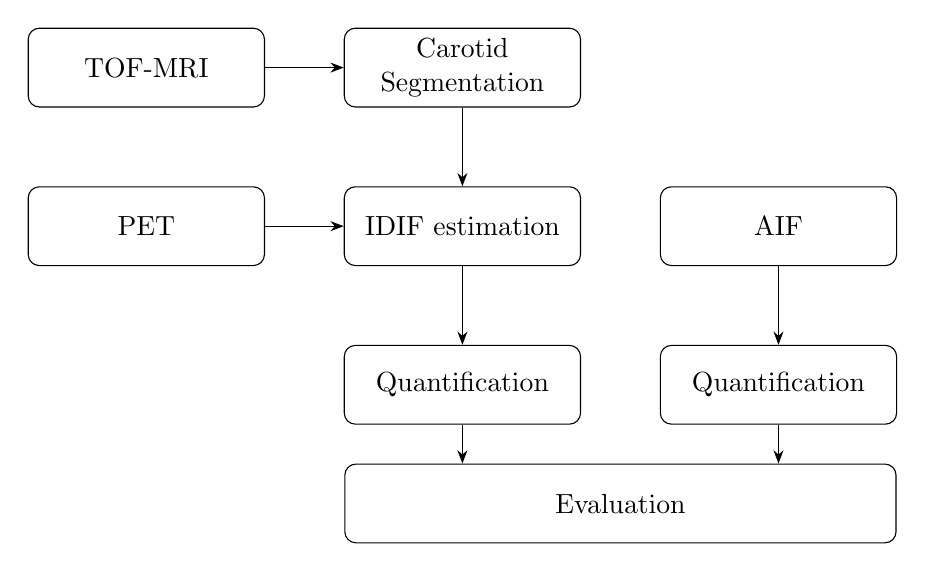
\begin{tikzpicture}[
			node distance=1cm,
			auto,
			>=Stealth,
			nodebox/.style={draw, rounded corners, rectangle, minimum width=3cm, minimum height=1cm, align=center}
		]
		\node[nodebox] (tof) {TOF-MRI};
		\node[nodebox, right=of tof] (seg) {Carotid\\Segmentation};
		\node[nodebox, below=of seg] (idif) {IDIF estimation};
		\node[nodebox, left=of idif] (pet) {PET};
		\node[nodebox, right=of idif] (aif) {AIF};
		\node[nodebox, below=of idif] (quantIDIF) {Quantification};
		\node[nodebox, below=of aif] (quantAIF) {Quantification};

		\coordinate (mid) at ($(quantIDIF)!0.5!(quantAIF)$);
		\node[nodebox,minimum width=7cm, below=of mid] (eval) {Evaluation};

		\draw[->] (tof) -- (seg);
		\draw[->] (seg) -- (idif);
		\draw[->] (pet) -- (idif);
		\draw[->] (idif) -- (quantIDIF);
		\draw[->] (aif) -- (quantAIF);
		\draw[->] (quantIDIF.south) -- (quantIDIF.south |- eval.north);
		\draw[->] (quantAIF.south) -- (quantAIF.south |- eval.north);
	\end{tikzpicture}
	\caption{The IDIF estimation and evaluation pipeline}
\end{figure}



\input{src/implementation}
\chapter{Results}
\section{Segmentation}
The measures described in Section~\ref{sec:carotid} significantly improved carotid segmentation by effectively excluding brain lesions and undesired venous structures.
As illustrated in Figure~\ref{fig:seg_compare}, the cuboid mask plays a crucial role in this process.
Because no ground truth segmentation is available, visual inspection was used to evaluate the results, which showed that lesions and venous structures were rarely selected by the algorithm.
However, the algorithm was sometimes overly conservative.
In some instances, even when no non-carotid tissues were selected, parts of the carotid were inadvertently excluded.

\begin{figure}[h]
	\centering
	\begin{subfigure}{0.45\textwidth}
		\includegraphics[width=\textwidth]{figures/molgu07704_bbox.png}
		\caption{}
		\label{subfig:seg_bbox}
	\end{subfigure}
	\begin{subfigure}{0.45\textwidth}
		\includegraphics[width=\textwidth]{figures/molgu07704_nobbox.png}
		\caption{}
		\label{subfig:seg_nobbox}
	\end{subfigure}
	\caption{Comparison of carotid segmentation (green) with (a) and without (b) a cuboid mask (yellow). In the absence of the cuboid mask, the segmentation algorithm fails to capture the carotid and instead incorrectly identifies the brain lesion}
	\label{fig:seg_compare}
\end{figure}

\section{IDIF}
IDIF estimation was performed using both the Bayesian GTM (BGTM) and the conventional GTM PVC method.
The average mean absolute error (MAE) of the cumulative area under the curve (cAUC) across the dataset was 14,202 for BGTM and 33,764 for GTM.

ROI-based quantification was carried out using both IDIF methods, with BGTM yielding significantly better performance.
Specifically, the BGTM and GTM methods achieved an average \(\mrglu\) mean absolute percentage error (MAPE) of 14.1\% and 33\%, respectively, and an average \(\mrglu\) mean absolute error (MAE) of 1.42 and 3.5.
In addition, the MAE for the coefficient of determination (\(R^2\)) and the regression slope (\(S\)) were 0.004 and 0.14 for BGTM, compared to 0.030 and 0.304 for GTM, respectively.


\begin{table}[h]
	\centering
	\begin{tabular}{l|cc|cc}
		\toprule
		\multirow{2}{*}{\textbf{Metric}} & \multicolumn{2}{c|}{\textbf{BGTM}} & \multicolumn{2}{c}{\textbf{GTM}}                        \\
		\cmidrule(lr){2-3} \cmidrule(lr){4-5}
		                                 & \(\mu\)                            & \(\sigma\)                       & \(\mu\) & \(\sigma\) \\
		\midrule
		cAUC MAE                         & 14,202                             & 9,190                            & 33,764  & 21,212     \\
		\(\textrm{MR}_{glu}\) MAPE (\%)  & \textbf{14.1}                      & \textbf{10.1}                    & 33.0    & 31.5       \\
		\(\textrm{MR}_{glu}\) MAE        & 1.42                               & 1.07                             & 3.50    & 3.38       \\
		\(R^2\) Error                    & 0.004                              & 0.006                            & 0.030   & 0.132      \\
		Slope Error                      & 0.14                               & 0.109                            & 0.304   & 0.230      \\
		\bottomrule
	\end{tabular}
	\caption{Summary of performance metrics for BGTM and GTM methods.}
	\label{tab:metrics}
\end{table}

\begin{figure}[h]
	\centering
	\begin{subfigure}[b]{0.45\textwidth}
		\includegraphics[width=\textwidth]{figures/quantification_mape_fitk3_boxplot.png}
		\caption{\(\mrglu\) MAPE Boxplot}
		\label{subfig:fitk3_mape}
	\end{subfigure}
	\begin{subfigure}[b]{0.45\textwidth}
		\includegraphics[width=\textwidth]{figures/curve_errors_boxplots.png}
		\caption{cAUC MAE Boxplot}
		\label{subfig:curve_errors_boxplot}
	\end{subfigure}
	\label{fig:boxplots}
	\caption{Boxplot of curve and quantification errors}
\end{figure}

As illustrated in Figure~\ref{fig:corr_mat}, there is a strong correlation between the MAE of the cAUC error and the quantification errors showing cAUC can be a good intermediate metric.
\pdfcomment{Consider whether additional analyses or details should be included to further support these results.}

\begin{figure}[h]
	\centering
	\begin{subfigure}{0.45\textwidth}
		\includegraphics[width=\textwidth]{figures/corr_gtm.png}
		\caption{GTM}
		\label{subfig:corr_gtm}
	\end{subfigure}
	\begin{subfigure}{0.45\textwidth}
		\includegraphics[width=\textwidth]{figures/corr_bgtm.png}
		\caption{Bayesian GTM}
		\label{subfig:corr_bgtm}
	\end{subfigure}
	\label{fig:corr_mat}
	\caption{Correlation matrix of different metrics for Bayesian GTM and GTM methods}
\end{figure}
\begin{figure}
	\centering
	\includegraphics[width=0.55\textwidth]{figures/RD11934_1_cmrglu.png}
	\caption{\(\mrglu\) regression line for a specific subject}
\end{figure}
\begin{figure}
	\centering
	\begin{subfigure}{\textwidth}
		\includegraphics[width=\textwidth]{figures/RD11934_1_if_comparison.png}
		% \caption{Input function comparison}
		\label{subfig:if_compare}
	\end{subfigure}
	\begin{subfigure}{\textwidth}
		\includegraphics[width=\textwidth]{figures/RD11934_1_trap.png}
		% \caption{Cumulative AUC of IFs}
		\label{subfig:trap_compare}
	\end{subfigure}
	\label{fig:ifs}
	\caption{Comparison of the IFs (Top) and Cumulative AUC curves (Bottom) for a specific subject}
\end{figure}



\chapter{Discussion}
% In this study, we proposed improvement
implemented and evaluated a method for estimating the image-derived arterial input function (IDIF) in brain PET imaging using multimodal MRI-PET data

\chapter{Conclusion}
This study demonstrates that combining TOF-MRA-guided carotid segmentation with Bayesian partial volume correction improves non-invasive input function estimation for PET/MRI in comatose patients.
While the method reduces reliance on invasive sampling, residual variability underscores challenges in spill-over correction and registration accuracy between PET and MR-derived vascular masks.
Future validation must address limitations in the current PCA framework by establishing standardized reference cohorts and expanding to multi-center studies with diverse patient populations.
By refining anatomical alignment protocols and ensuring consistent prior knowledge integration, this approach can enhance reliability for clinical translation, ultimately supporting safer, patient-friendly quantitative PET imaging.

\newpage
\fancyhead{}
\fancyhead[L]{\textsc{References}}
\printbibliography[
	heading=bibintoc,
	title={References}]



\end{document}

